%============================================================
%  AUTHORIZATION DENIAL DATA INTELLIGENCE PROPOSAL
%  COB Solutions → PT of the City
%  Author: Abdelrahman Hamdy — AI / COB Solutions
%  Compile: pdflatex x2
%============================================================
\documentclass[11pt,a4paper]{article}

\usepackage[T1]{fontenc}
\usepackage[utf8]{inputenc}
\usepackage{mathptmx}
\usepackage[scaled=0.92]{helvet}
\usepackage{courier}
\usepackage{microtype}
\usepackage[top=2.5cm,bottom=2.5cm,left=2.5cm,right=2.5cm,headheight=16pt]{geometry}
\usepackage{xcolor}
\usepackage{graphicx}
\usepackage{amsmath}
\usepackage{booktabs}
\usepackage{array}
\usepackage{colortbl}
\usepackage{multicol}
\usepackage{enumitem}
\usepackage{fancyhdr}
\usepackage{titlesec}
\usepackage{tcolorbox}
\usepackage{tikz}
\usepackage{hyperref}
\usepackage{tabularx}
\usepackage{longtable}

\usetikzlibrary{shapes.geometric,arrows.meta,positioning,fit,calc,shadows,backgrounds}
\tcbuselibrary{skins,breakable}

%-----------------------------------------------------------
% COLOURS
%-----------------------------------------------------------
\definecolor{PrimaryBlue}{HTML}{1A3C5E}
\definecolor{AccentTeal}{HTML}{0D7C8C}
\definecolor{AccentGold}{HTML}{C8962A}
\definecolor{LightBg}{HTML}{F4F7FA}
\definecolor{MidGray}{HTML}{6B7B8D}
\definecolor{DangerRed}{HTML}{C0392B}
\definecolor{SuccessGreen}{HTML}{1E8449}
\definecolor{WarningAmber}{HTML}{D4850A}
\definecolor{SoftBlue}{HTML}{D6E4F0}
\definecolor{SoftTeal}{HTML}{D0EEF2}
\definecolor{SoftGold}{HTML}{FAF0DC}
\definecolor{SoftRed}{HTML}{FADBD8}
\definecolor{SoftGreen}{HTML}{D5F5E3}
\definecolor{TableHead}{HTML}{1A3C5E}
\definecolor{TableAlt}{HTML}{EAF2FA}
\definecolor{RuleColor}{HTML}{B0C4D8}

%-----------------------------------------------------------
% HYPERREF
%-----------------------------------------------------------
\hypersetup{colorlinks=true,linkcolor=PrimaryBlue,urlcolor=AccentTeal,
  pdftitle={Authorization Denial Data --- Solution Proposal --- COB Solutions},
  bookmarksnumbered=true}

%-----------------------------------------------------------
% HEADER / FOOTER
%-----------------------------------------------------------
\pagestyle{fancy}\fancyhf{}
\fancyhead[L]{\color{MidGray}\small\textit{COB Solutions --- Authorization Denial Data}}
\fancyfoot[C]{\color{MidGray}\thepage}
\renewcommand{\headrulewidth}{0.4pt}
\renewcommand{\headrule}{\hbox to\headwidth{\color{RuleColor}\leaders\hrule height\headrulewidth\hfill}}

%-----------------------------------------------------------
% SECTION STYLING
%-----------------------------------------------------------
\titleformat{\section}{\color{PrimaryBlue}\Large\bfseries}
  {\colorbox{PrimaryBlue}{\color{white}\ \thesection\ }}{0.8em}{}
  [\vspace{-0.2em}\color{RuleColor}\rule{\linewidth}{1.5pt}\vspace{0.3em}]
\titleformat{\subsection}{\color{AccentTeal}\large\bfseries}
  {\color{AccentTeal}\thesubsection}{0.6em}{}
  [\vspace{-0.3em}\color{RuleColor}\rule{\linewidth}{0.6pt}]
\titleformat{\subsubsection}{\color{PrimaryBlue}\normalsize\bfseries}
  {\color{AccentGold}\thesubsubsection}{0.5em}{}
\titlespacing*{\section}{0pt}{1.6em}{0.8em}
\titlespacing*{\subsection}{0pt}{1.2em}{0.5em}
\titlespacing*{\subsubsection}{0pt}{0.9em}{0.3em}

%-----------------------------------------------------------
% LISTS
%-----------------------------------------------------------
\setlist[itemize,1]{label={\color{AccentTeal}\textbullet},leftmargin=1.5em,itemsep=0.25em,topsep=0.3em}
\setlist[itemize,2]{label={\color{AccentGold}\small$\blacktriangleright$},leftmargin=1.5em,itemsep=0.15em}
\setlist[enumerate,1]{label={\color{PrimaryBlue}\bfseries\arabic*.},leftmargin=1.8em,itemsep=0.25em}

%-----------------------------------------------------------
% TCOLORBOX STYLES
%-----------------------------------------------------------
\tcbset{
  infobox/.style={enhanced,breakable,colback=SoftBlue,colframe=PrimaryBlue,
    boxrule=1.2pt,arc=4pt,left=8pt,right=8pt,top=6pt,bottom=6pt,
    fonttitle=\bfseries\color{white},
    attach boxed title to top left={yshift=-2mm,xshift=6mm},
    boxed title style={colback=PrimaryBlue,arc=3pt,boxrule=0pt}},
  warnbox/.style={enhanced,breakable,colback=SoftGold,colframe=WarningAmber,
    boxrule=1.2pt,arc=4pt,left=8pt,right=8pt,top=6pt,bottom=6pt,
    fonttitle=\bfseries\color{white},
    attach boxed title to top left={yshift=-2mm,xshift=6mm},
    boxed title style={colback=WarningAmber,arc=3pt,boxrule=0pt}},
  successbox/.style={enhanced,breakable,colback=SoftGreen,colframe=SuccessGreen,
    boxrule=1.2pt,arc=4pt,left=8pt,right=8pt,top=6pt,bottom=6pt,
    fonttitle=\bfseries\color{white},
    attach boxed title to top left={yshift=-2mm,xshift=6mm},
    boxed title style={colback=SuccessGreen,arc=3pt,boxrule=0pt}},
  dangerbox/.style={enhanced,breakable,colback=SoftRed,colframe=DangerRed,
    boxrule=1.2pt,arc=4pt,left=8pt,right=8pt,top=6pt,bottom=6pt,
    fonttitle=\bfseries\color{white},
    attach boxed title to top left={yshift=-2mm,xshift=6mm},
    boxed title style={colback=DangerRed,arc=3pt,boxrule=0pt}},
  statbox/.style={enhanced,colback=LightBg,colframe=AccentGold,
    boxrule=2pt,arc=6pt,left=10pt,right=10pt,top=8pt,bottom=8pt},
  rulebox/.style={enhanced,breakable,colback=LightBg,colframe=PrimaryBlue,
    boxrule=0.8pt,arc=3pt,left=7pt,right=7pt,top=6pt,bottom=6pt,
    borderline west={3pt}{0pt}{AccentTeal}}
}

%-----------------------------------------------------------
% TIKZ BASE STYLES
%-----------------------------------------------------------
\tikzset{
  FB/.style={rectangle,rounded corners=3pt,
             minimum width=2.1cm,minimum height=0.75cm,
             text centered,align=center,draw,thick,
             font=\scriptsize\bfseries},
  arr/.style={-{Stealth[length=4.5pt]},thick},
  nB/.style={FB,fill=SoftBlue, draw=PrimaryBlue,text=PrimaryBlue},
  nT/.style={FB,fill=SoftTeal, draw=AccentTeal, text=AccentTeal},
  nG/.style={FB,fill=SoftGold, draw=AccentGold, text=AccentGold},
  nV/.style={FB,fill=SoftGreen,draw=SuccessGreen,text=SuccessGreen},
  nR/.style={FB,fill=SoftRed,  draw=DangerRed,  text=DangerRed}
}

%-----------------------------------------------------------
% HELPERS
%-----------------------------------------------------------
\newcolumntype{L}[1]{>{\raggedright\arraybackslash}p{#1}}
\newcolumntype{C}[1]{>{\centering\arraybackslash}p{#1}}
\newcommand{\statusReuse}{\textcolor{SuccessGreen}{\textbf{Reusable core}}}
\newcommand{\statusPartial}{\textcolor{AccentGold}{\textbf{Partial}}}
\newcommand{\statusBuild}{\textcolor{DangerRed}{\textbf{To build}}}
\newcommand{\statusTrans}{\textcolor{AccentTeal}{\textbf{Transitional}}}

%============================================================
\begin{document}
%============================================================

%------------------------------------------------------------
% COVER PAGE
%------------------------------------------------------------
\begin{titlepage}
\pagecolor{PrimaryBlue}\color{white}
\vspace*{0.6cm}
\begin{center}
  \textcolor{AccentGold}{\rule{0.88\linewidth}{2pt}}\\[0.3em]
  \textcolor{AccentGold}{\rule{0.88\linewidth}{0.5pt}}\\[1.4cm]

  {\fontsize{14}{18}\selectfont\color{SoftBlue}\textsc{COB Solutions}}\\[0.4em]
  {\fontsize{12}{16}\selectfont\color{AccentGold}\textbf{Prepared for PT of the City}}\\[0.3em]
  {\fontsize{11}{14}\selectfont\color{SoftBlue}Clinical Performance \textbullet{} RCM \textbullet{} AI Team}\\[1.2cm]

  {\fontsize{26}{32}\selectfont\bfseries Authorization Denial}\\[0.15em]
  {\fontsize{26}{32}\selectfont\bfseries Data Intelligence}\\[0.5em]
  {\fontsize{16}{20}\selectfont\color{AccentGold}Solution Proposal}\\[0.8em]

  \textcolor{AccentGold}{\rule{0.5\linewidth}{0.8pt}}\\[0.6em]
  {\color{SoftBlue}\small
    Daily Denial Extract \textbullet{} Letter Completeness \textbullet{}
    Reason Classification \textbullet{} Visit KPIs}\\[1.6cm]

  {\color{SoftBlue}\normalsize
    Response to Clinical Performance requirements\\[0.3em]
    Meeting thread: 23--28 July 2026}\\[0.8cm]

  {\color{AccentGold}\textbf{Author:} Eng.\ Abdelrahman Hamdy --- AI / COB Solutions}

  \vfill
  \textcolor{AccentGold}{\rule{0.88\linewidth}{0.5pt}}\\[0.3em]
  \textcolor{AccentGold}{\rule{0.88\linewidth}{2pt}}
\end{center}
\end{titlepage}
\nopagecolor\color{black}

%------------------------------------------------------------
% TABLE OF CONTENTS
%------------------------------------------------------------
\newpage
\tableofcontents
\newpage

%============================================================
\section{Executive Summary}
%============================================================

\subsection{Current challenge}

Authorization denials today are tracked across five cluster Workload sheets and patient
charts. Teams lack a reliable daily view of which Denied requests are missing an uploaded
denial letter, why the denial occurred, and how much visit volume sits behind those
denials. Manual lookup slows Clinical Performance and RCM action.

\subsection{Proposed solution}

\textbf{COB Solutions / AI Team} will deliver a daily Authorization Denial dataset that:

\begin{itemize}
  \item Pulls Denied rows from the five PTOC cluster authorization sheets (since May 2026).
  \item Links each row to the correct Case Name / Case ID from finalized clinical notes.
  \item Checks whether a denial letter is on the chart (File Name, or
        \texttt{Not Found in the File Name}).
  \item When a letter is present: extracts the raw description, decision date, and reason
        category---including Missing Referral.
  \item Reports defined visit KPIs on the denied cohort only---not vanity averages.
\end{itemize}

\subsection{Business outcome}

\begin{tcolorbox}[statbox]
\begin{center}
  \Large\bfseries\color{PrimaryBlue}Primary Return on Effort\\[0.5em]
\end{center}
Primary ROI is RCM and Clinical Performance time redirected from chart hunting to
exception handling and root-cause action. Secondary ROI is faster letter completeness
and payer-focused denial reduction using defined KPIs---not vanity averages.
\end{tcolorbox}

\subsection{Delivery note}

The AI team will automate this end-to-end extract on a daily schedule. Existing
letter-reading capability will be wired into the full Patient~$\rightarrow$~Case~$\rightarrow$~Letter
workflow. Cluster authorization sheets remain the source until the new denial management
system (Kareem Kholy) is live.


%============================================================
\section{Business Objectives}
%============================================================

\subsection{What Clinical Performance and RCM receive}

\begin{enumerate}
  \item \textbf{Patient list} --- A daily denial list from all five cluster Workload tabs
        (\texttt{Request Status = Denied}, since May 2026), including Patient ID, DOS, and
        Location Name.
  \item \textbf{Case} --- Case Name / Case ID linked from Patient ID + Date of Service to
        the finalized clinical note; rows that cannot be confidently matched are flagged
        for review (no guessing).
  \item \textbf{Letter} --- Denial-letter status per row: File Name when present, or
        \texttt{Not Found in the File Name} when absent.
  \item \textbf{Extract} --- When a letter is found: raw description and decision date,
        then Reason Category (including Missing Referral), with Insurance Name and ICD-10
        for clinical context.
  \item \textbf{Analytics} --- Visit KPIs with explicit definitions on the denied cohort only.
  \item \textbf{Validation} --- A stratified sample for RCM review of AI-generated
        description and category.
\end{enumerate}

\subsection{Source sheets}

\begin{itemize}
  \item PTOC --- Queens Cluster Authorization Sheet
  \item PTOC --- Bronx Cluster Authorization Sheet
  \item PTOC --- Upper Brooklyn Cluster Authorization Sheet
  \item PTOC --- Lower Brooklyn Cluster Authorization Sheet 2026
  \item PTOC --- Manhattan Cluster Authorization Sheet
\end{itemize}

These sheets are updated daily and will be used until the new denial management system
is live. Exact clock time of the daily refresh remains an open ask so the AI extract can
run safely afterward.


%============================================================
\section{Business Value, KPIs \& ROI}
%============================================================

\subsection{Pain today}

\begin{itemize}
  \item Manual hunting across five cluster sheets and patient charts for Denied rows.
  \item No reliable daily view of which denials lack an uploaded letter.
  \item Reason categories not systematically extracted---hard to coach or trend.
  \item Visit analytics for the denied cohort are ad hoc and undefined
        (denominator unclear: all payer patients vs.\ denial patients only).
\end{itemize}

\subsection{Value levers after delivery}

\begin{tcolorbox}[successbox,title={What this solution unlocks}]
\begin{enumerate}
  \item \textbf{Root-cause clarity} --- Categorized reasons (including Missing Referral)
        show \emph{why} denials happen---referral workflow vs.\ documentation vs.\ medical
        necessity---so coaching and process fixes are targeted, not generic.
  \item \textbf{Labor time saved} --- Replace repetitive sheet~$\rightarrow$~chart~$\rightarrow$~filename
        checks with a daily automated extract. Teams review exceptions and validation
        samples instead of 100\% manual lookup.
  \item \textbf{Faster missing-letter remediation} ---
        \texttt{Not Found in the File Name} becomes an actionable queue
        (upload letter~$\rightarrow$~unlock appeal and classification).
  \item \textbf{Payer / visit exposure} --- Defined KPIs show which insurers and cases
        carry the most visit burden under denial---supports staffing and escalation.
  \item \textbf{Validation loop} --- AI proposes description and category; RCM samples
        for accuracy without reading every letter.
  \item \textbf{Ready for the new denial system} --- Case, letter, and category logic stay
        in place when sheets are replaced---work is not thrown away.
\end{enumerate}
\end{tcolorbox}

\subsection{Visit analytics KPIs --- definitions}

Clinic-wide payer averages (all patients of an insurance) are \textbf{out of scope /
Phase~2}. MVP KPIs use the \textbf{authorization-denied cohort only}.

\begin{table}[h!]
\centering
\renewcommand{\arraystretch}{1.25}
\begin{tabularx}{\linewidth}{L{3.2cm} X L{3.4cm}}
\toprule
\rowcolor{TableHead}
\textcolor{white}{\bfseries KPI} &
\textcolor{white}{\bfseries Definition} &
\textcolor{white}{\bfseries Decision enabled} \\
\midrule
Total visits per case &
Count of completed / checked-out visits on the \textbf{resolved Case} for each denied
authorization row. Source: chart visit fields and/or schedule/checkout history for that case. &
Prioritize appeals vs.\ stop; flag high-visit cases stuck without a letter \\
\rowcolor{TableAlt}
Avg.\ visits per insurance (denied cohort) &
Average visits per case for \textbf{denied rows only}, by Insurance Name
(not clinic-wide payer volume). &
Focus documentation / referral prep on high-burden payers \\
Avg.\ sessions per case (denial patients) &
Average clinical visits per denied case, counted through the denial decision date. &
Capacity \& clinical performance baseline before process improvements \\
\bottomrule
\end{tabularx}
\caption{Visit KPIs: definition and management use.}
\end{table}

\subsection{Operational KPIs (pipeline health)}

\begin{table}[h!]
\centering
\renewcommand{\arraystretch}{1.2}
\begin{tabularx}{\linewidth}{L{4.2cm} X}
\toprule
\rowcolor{TableHead}
\textcolor{white}{\bfseries Ops KPI} &
\textcolor{white}{\bfseries Why it matters} \\
\midrule
\% rows \texttt{Not Found in the File Name} &
Missing-letter backlog; blocks appeals and classification \\
\rowcolor{TableAlt}
\% \texttt{Case\_Ambiguous} / unmatched &
Mapping debt; prevents silent wrong joins \\
Reason-category mix (incl.\ Missing Referral) &
Root-cause view for Clinical Performance and RCM coaching \\
\rowcolor{TableAlt}
Daily refresh lag (hours after sheet update) &
Trust in the denial list for same-day action \\
\bottomrule
\end{tabularx}
\caption{Operational KPIs from the daily pipeline.}
\end{table}

\subsection{ROI assumptions (no fabricated dollars)}

We do not invent a dollar ROI without PT of the City volume and effort inputs.
After the first 1--2 weeks of production extracts, the AI team will estimate time saved
using simple operational assumptions---not a finance model that managers must calculate.

\begin{tcolorbox}[infobox,title={ROI assumptions}]
\textbf{Time saved} will be estimated from:\\[0.3em]
denied volume $\times$ minutes of manual work per row today $\times$ share of rows handled
automatically (excluding rows flagged for human review).\\[0.4em]
\textbf{Also counted as value (not only minutes):} fewer missed missing-letter cases,
faster appeal readiness, and clearer payer-specific coaching from reason mix and visit KPIs.
\end{tcolorbox}

\begin{table}[h!]
\centering
\renewcommand{\arraystretch}{1.2}
\begin{tabularx}{\linewidth}{L{5.5cm} C{3.5cm} X}
\toprule
\rowcolor{TableHead}
\textcolor{white}{\bfseries Assumption input} &
\textcolor{white}{\bfseries Placeholder} &
\textcolor{white}{\bfseries Owner} \\
\midrule
Denied volume per week (approx.) & \textit{TBD} & RCM / Clinical Performance \\
\rowcolor{TableAlt}
Est.\ minutes per row today & \textit{TBD} & RCM \\
Loaded staff cost per hour (optional) & \textit{TBD} & Finance / Ops \\
\rowcolor{TableAlt}
Share handled automatically after MVP & e.g.\ 70--85\% & AI + RCM jointly \\
\bottomrule
\end{tabularx}
\caption{Inputs to refine after first production weeks.}
\end{table}


%============================================================
\section{Scope \& Data Contract}
%============================================================

\subsection{Output fields}

\begin{table}[h!]
\centering
\renewcommand{\arraystretch}{1.15}
\begin{tabularx}{\linewidth}{L{4.0cm} X L{2.4cm}}
\toprule
\rowcolor{TableHead}
\textcolor{white}{\bfseries Field} &
\textcolor{white}{\bfseries Notes} &
\textcolor{white}{\bfseries Source} \\
\midrule
Patient ID & From Workload Denied row & Sheets \\
\rowcolor{TableAlt}
Date of Service (DOS) & Visit DOS on denied request & Sheets \\
Location Name & Cluster / clinic location & Sheets \\
\rowcolor{TableAlt}
Case ID / Case Name & Via Case Resolution Strategy & WebPT \\
Filename / letter status & File Name or \texttt{Not Found in the File Name} & Chart eDocs \\
\rowcolor{TableAlt}
Denial Date (decision date) & From letter text when letter found & Letter extract \\
Submitted note date / DOS & Align with sheet DOS; note date may differ & Sheets / notes \\
\rowcolor{TableAlt}
Insurance Name & Sheet and/or letter & Sheets / letter \\
ICD-10 Code & Sheet if present; else chart diagnosis & Sheets / chart \\
\rowcolor{TableAlt}
Denial letter description (raw) & Full extracted reason text & Letter extract \\
Reason Category & See categories below & Classifier \\
\rowcolor{TableAlt}
Denial letter upload date & If available from chart document metadata & Chart eDocs \\
Resolution Status & Matched / Case Ambiguous / Case Not Found & Pipeline \\
\bottomrule
\end{tabularx}
\caption{Denial dataset data contract.}
\end{table}

\subsection{Reason categories}

Agreed clinical categories:

\begin{itemize}
  \item Skilled care not supported
  \item Documentation insufficient
  \item Medical necessity
  \item Visit limit or benefit
  \item Missing Referral --- captured through payer language variants
        (e.g.\ referral required, not on file, expired, PCP referral required)
\end{itemize}


%============================================================
\section{Solution Approach}
%============================================================

\subsection{Daily flow}

\begin{figure}[h!]
\centering
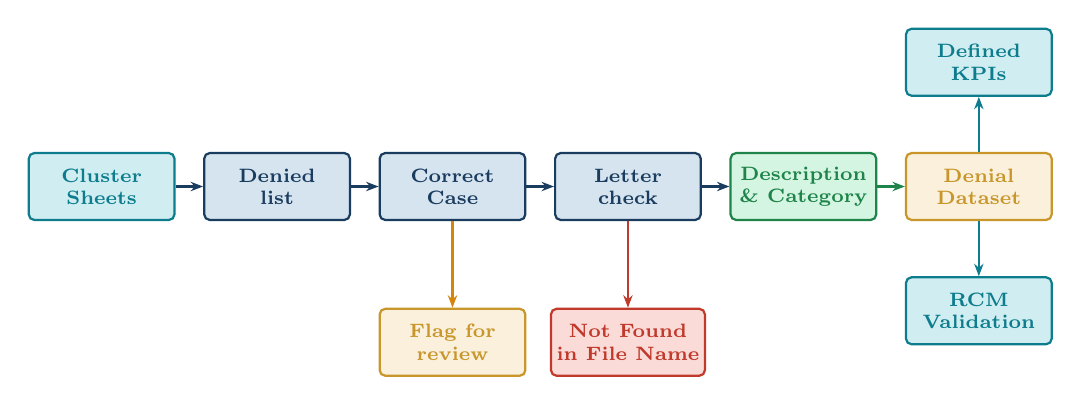
\begin{tikzpicture}[
  node distance=0.45cm and 0.35cm,
  every node/.style={font=\scriptsize\bfseries},
  box/.style={rectangle,rounded corners=2pt,draw,thick,align=center,
              minimum height=0.85cm,minimum width=1.85cm,inner sep=2pt}
]
  \node[box,fill=SoftTeal,draw=AccentTeal,text=AccentTeal] (s1) {Cluster\\Sheets};
  \node[box,fill=SoftBlue,draw=PrimaryBlue,text=PrimaryBlue,right=of s1] (s2) {Denied\\list};
  \node[box,fill=SoftBlue,draw=PrimaryBlue,text=PrimaryBlue,right=of s2] (s3) {Correct\\Case};
  \node[box,fill=SoftGold,draw=AccentGold,text=AccentGold,below=1.1cm of s3] (amb) {Flag for\\review};
  \node[box,fill=SoftBlue,draw=PrimaryBlue,text=PrimaryBlue,right=of s3] (s4) {Letter\\check};
  \node[box,fill=SoftRed,draw=DangerRed,text=DangerRed,below=1.1cm of s4] (nf) {Not Found\\in File Name};
  \node[box,fill=SoftGreen,draw=SuccessGreen,text=SuccessGreen,right=of s4] (s5) {Description\\\& Category};
  \node[box,fill=SoftGold,draw=AccentGold,text=AccentGold,right=of s5] (s6) {Denial\\Dataset};
  \node[box,fill=SoftTeal,draw=AccentTeal,text=AccentTeal,above=0.7cm of s6] (an) {Defined\\KPIs};
  \node[box,fill=SoftTeal,draw=AccentTeal,text=AccentTeal,below=0.7cm of s6] (va) {RCM\\Validation};

  \draw[arr,PrimaryBlue] (s1) -- (s2);
  \draw[arr,PrimaryBlue] (s2) -- (s3);
  \draw[arr,PrimaryBlue] (s3) -- (s4);
  \draw[arr,WarningAmber] (s3) -- (amb);
  \draw[arr,PrimaryBlue] (s4) -- (s5);
  \draw[arr,DangerRed] (s4) -- (nf);
  \draw[arr,SuccessGreen] (s5) -- (s6);
  \draw[arr,AccentTeal] (s6) -- (an);
  \draw[arr,AccentTeal] (s6) -- (va);
\end{tikzpicture}
\caption{Daily flow from cluster sheets to KPIs and RCM validation.}
\end{figure}

\subsection{Phase A --- Sheets intake}

\begin{itemize}
  \item Read the \textbf{Workload} tab on each of the five cluster authorization sheets.
  \item Keep rows where \texttt{Request Status = Denied} (since May 2026).
  \item Capture Patient ID, DOS, Location Name, and any insurance / ICD columns available.
  \item When the new denial management system replaces the sheets, the same case / letter /
        category steps continue without starting over.
\end{itemize}

\subsection{Phase B --- Linking the correct case}

Each Denied row is linked to the Case Name associated with the finalized note for that
patient and date of service. When more than one case or note could apply, the row is
\textbf{flagged for review} instead of assigning a guess.

\begin{figure}[h!]
\centering
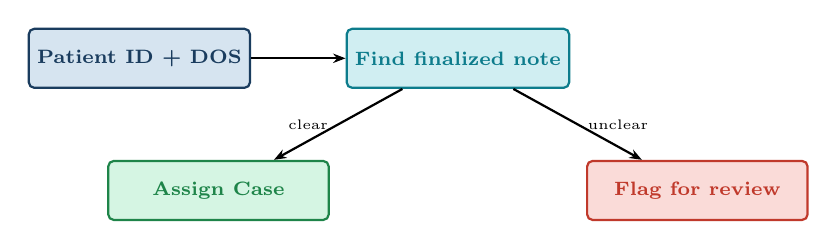
\begin{tikzpicture}[
  node distance=0.7cm and 1.2cm,
  every node/.style={font=\scriptsize\bfseries},
  box/.style={rectangle,rounded corners=2pt,draw,thick,align=center,
              minimum height=0.75cm,minimum width=2.8cm,inner sep=3pt}
]
  \node[box,fill=SoftBlue,draw=PrimaryBlue,text=PrimaryBlue] (a) {Patient ID + DOS};
  \node[box,fill=SoftTeal,draw=AccentTeal,text=AccentTeal,right=of a] (b) {Find finalized note};
  \node[box,fill=SoftGreen,draw=SuccessGreen,text=SuccessGreen,below left=0.9cm and 0.2cm of b] (c) {Assign Case};
  \node[box,fill=SoftRed,draw=DangerRed,text=DangerRed,below right=0.9cm and 0.2cm of b] (d) {Flag for review};

  \draw[arr] (a) -- (b);
  \draw[arr] (b) -- node[left,font=\tiny]{clear} (c);
  \draw[arr] (b) -- node[right,font=\tiny]{unclear} (d);
\end{tikzpicture}
\caption{Case linking: assign when clear; flag when ambiguous.}
\end{figure}

\subsection{Phase C --- Denial letter check and extract}

\begin{enumerate}
  \item Check the patient chart for a denial letter on the matched case.
  \item If none: set status \texttt{Not Found in the File Name}.
  \item If found: record the File Name and extract the raw description, decision date,
        and Reason Category.
\end{enumerate}

\subsection{Phase D --- Missing Referral}

Missing Referral is a required clinical category. The extract will recognize common payer
wording such as: referral required, referral missing, not on file, not received,
PCP referral required, referral expired, or referral invalid. RCM will validate a sample
focused on this category so coaching stays accurate.

\subsection{Phase E --- Analytics}

Produce the visit KPIs and operational KPIs defined earlier (denied cohort only), plus
exception queues for missing letters and ambiguous cases.

\subsection{Phase F --- Daily refresh and validation sample}

\begin{itemize}
  \item Run after the daily sheet update (time to be confirmed by RCM).
  \item Deliver the full denial dataset plus exception queues.
  \item Deliver a stratified validation sample (including Missing Referral) for RCM review.
\end{itemize}


%============================================================
\section{Capability Inventory}
%============================================================

\textit{For delivery planning (AI / management):} what already exists versus what we will
build for this workflow. Clinical Performance readers can skip this section; outcomes are
covered above.

\begin{tcolorbox}[warnbox,title={Status legend}]
\statusReuse{} --- letter-reading / classification capability exists; used after the correct
denial letter is identified.\\
\statusPartial{} --- supporting fields or APIs exist but are not yet wired into this daily flow.\\
\statusBuild{} --- end-to-end wiring still required for this deliverable.\\
\statusTrans{} --- sheets as source until the new denial management system replaces them.
\end{tcolorbox}

\begin{tcolorbox}[rulebox,title={Delivery note for planning}]
Description, decision date, and reason category are produced by a \statusReuse{}
\textbf{after} Patient~$\rightarrow$~Case~$\rightarrow$~correct Letter are resolved.
Upstream discovery and letter selection are \statusBuild{}. This is planning language---not
a claim that the full daily pipeline is already finished.
\end{tcolorbox}

\begin{table}[h!]
\centering
\renewcommand{\arraystretch}{1.2}
\begin{tabularx}{\linewidth}{L{4.6cm} L{2.6cm} X}
\toprule
\rowcolor{TableHead}
\textcolor{white}{\bfseries Requirement} &
\textcolor{white}{\bfseries Status} &
\textcolor{white}{\bfseries Notes} \\
\midrule
Workload Denied extract (5 sheets) &
\statusBuild{} &
Sheet intake until new denial system \\
\rowcolor{TableAlt}
Patient ID, DOS, Location &
\statusBuild{} &
From sheets \\
Case Name via Finalized note &
\statusBuild{} &
Case linking + review flags; chart APIs = Partial \\
\rowcolor{TableAlt}
Letter presence / File Name / Not Found &
\statusBuild{} &
Chart check + status column; letter-find helpers = Reusable \\
Raw description, Decision Date, Category &
\statusReuse{} &
After correct letter selected---not a finished stage alone \\
\rowcolor{TableAlt}
Missing Referral + other categories &
Mixed &
Existing categories = Reusable; Missing Referral wording = To build \\
Visit KPIs (defined above) &
\statusBuild{} &
Visit fields on chart = Partial; denied-cohort rollups = To build \\
\rowcolor{TableAlt}
Daily refresh &
\statusBuild{} &
Schedule after sheet update time \\
\bottomrule
\end{tabularx}
\caption{Capability inventory for delivery planning.}
\end{table}


%============================================================
\section{Timeline \& Effort}
%============================================================

\begin{tcolorbox}[statbox]
\begin{center}
{\Large\bfseries\color{PrimaryBlue}Estimated duration: 10--12 working days}\\[0.4em]
{\normalsize Production daily MVP, plus $\sim$2 days buffer for sheet quirks and cutover prep.}
\end{center}
\end{tcolorbox}

\begin{table}[h!]
\centering
\renewcommand{\arraystretch}{1.25}
\begin{tabularx}{\linewidth}{C{2.2cm} L{3.0cm} X}
\toprule
\rowcolor{TableHead}
\textcolor{white}{\bfseries Window} &
\textcolor{white}{\bfseries Focus} &
\textcolor{white}{\bfseries Deliverables} \\
\midrule
Days 1--5 &
Intake + Case + Letter status &
Sheets connector; Denied extract; case linking; letter check; \texttt{Not Found in the File Name} \\
\rowcolor{TableAlt}
Days 6--9 &
Extract + Missing Referral &
Description / category extract in the daily flow; Missing Referral wording; insurance / ICD context; validation sample \\
Days 10--12 &
KPIs + daily ops &
Visit \& ops KPI reports; daily scheduler (after sheet refresh); handoff to Clinical Performance / RCM \\
\rowcolor{TableAlt}
Buffer (+2) &
Schema / cutover &
Sheet column changes; prep to switch intake when the new denial system is ready \\
\bottomrule
\end{tabularx}
\caption{Estimated phased delivery schedule.}
\end{table}

\begin{tcolorbox}[rulebox,title={Dependency}]
Daily job timing depends on confirmation of \textbf{what time of day} the authorization
sheets are typically updated. Until then, the job can run on a conservative evening
window or on-demand.
\end{tcolorbox}


%============================================================
\section{Assumptions \& Open Asks}
%============================================================

\begin{enumerate}
  \item \textbf{Sheet update clock time} --- needed from RCM (Kareem / owners) for safe
        scheduling.
  \item \textbf{Access} --- AI team read access to all five cluster authorization sheets
        (Workload tabs).
  \item \textbf{ICD-10} --- confirm whether Workload always carries ICD-10 or whether
        chart diagnosis is the fallback.
  \item \textbf{Case ID on sheet} --- if Workload already has a case identifier, use it
        as a strong hint inside Case Resolution; otherwise resolve solely from finalized notes.
  \item \textbf{ROI calibration inputs} --- denied volume/week and est.\ minutes per row
        from RCM after first production weeks.
  \item \textbf{KPI window} --- default is visits through denial decision date; Clinical
        Performance should confirm or request lifetime case visits as Phase~2.
  \item \textbf{New denial system} --- intake will switch when Kareem's system replaces
        Sheets; case, letter, and category steps stay.
\end{enumerate}


%============================================================
\section{Validation Plan}
%============================================================

\begin{itemize}
  \item AI generates denial description (raw) and Reason Category for rows with a found letter.
  \item RCM validates a \textbf{stratified sample} (by reason class and payer), with
        dedicated coverage of \texttt{missing\_referral} candidates.
  \item Feedback loops into pattern/classifier tuning (especially referral language and
        false positives vs.\ documentation / medical necessity).
  \item Exception queues (\texttt{Not Found in the File Name}, \texttt{Case\_Ambiguous})
        are operational outputs for remediation, not validation failures of the model.
\end{itemize}


%============================================================
\section{Risks \& Mitigations}
%============================================================

\begin{table}[h!]
\centering
\renewcommand{\arraystretch}{1.2}
\begin{tabularx}{\linewidth}{L{3.6cm} X X}
\toprule
\rowcolor{TableHead}
\textcolor{white}{\bfseries Risk} &
\textcolor{white}{\bfseries Impact} &
\textcolor{white}{\bfseries Mitigation} \\
\midrule
Multi-case / multi-note ambiguity &
Wrong Case Name &
Case Resolution Strategy; explicit Ambiguous flag; no silent pick \\
\rowcolor{TableAlt}
Wrong letter selected &
Wrong category / date &
Date proximity + filename/content rules; RCM sample review \\
OCR quality / scanned letters &
\texttt{unparseable} or weak reason &
Existing OCR path; re-queue; human sample on hard payers \\
\rowcolor{TableAlt}
Sheets column drift / cutover &
Broken intake &
Buffer days; switch intake when the new denial system is ready \\
Missing Referral false positives &
Mis-coaching &
Pattern pack + stratified validation focused on referral class \\
\bottomrule
\end{tabularx}
\caption{Key risks and mitigations.}
\end{table}


%============================================================
\section{Closing}
%============================================================

This solution gives Clinical Performance and RCM a daily view of authorization denials:
root-cause categories for coaching (including Missing Referral), a clear missing-letter
queue, correct case linkage, and defined visit KPIs on the denied cohort---so effort moves
from chart hunting to exceptions and action.

Time-saved estimates will be refined with real denied volume and minutes-per-row after the
first production weeks, not asserted with invented dollar figures.

\begin{tcolorbox}[statbox]
\begin{center}
{\bfseries\color{PrimaryBlue}Next steps}\\[0.5em]
\end{center}
\begin{enumerate}
  \item Confirm sheet update time and grant Sheets access.
  \item Confirm KPI window (through decision date vs.\ lifetime) and ICD-10 source.
  \item AI team begins Phase~A--B (intake + case linking) immediately after access.
  \item RCM prepares to validate the first stratified sample in Week~2.
\end{enumerate}
\end{tcolorbox}

\vspace{1.2em}
\begin{center}
\color{MidGray}\small
Prepared by Eng.\ Abdelrahman Hamdy --- AI / COB Solutions\\
For PT of the City --- Clinical Performance \& RCM\\
July 2026
\end{center}

\end{document}
